\documentclass[10pt,letterpaper]{article}

\usepackage{iclr2027_conference,times}
\usepackage[T1]{fontenc}
\usepackage[utf8]{inputenc}
\usepackage{microtype}
\usepackage{graphicx}
\usepackage{booktabs}
\usepackage{tabularx}
\usepackage{subcaption}
\usepackage{amsmath}
\usepackage{float}
\usepackage{placeins}
\usepackage{tikz}
\usetikzlibrary{arrows.meta,positioning,calc}
\usepackage[hidelinks]{hyperref}

% All Overleaf-ready PDF assets are kept in one flat figures/ directory.
\graphicspath{{figures/}{kd/figures/}}

\setlength{\parindent}{0pt}
\setlength{\parskip}{2.5pt}
\captionsetup{font=small,labelfont=bf}
\pagestyle{plain}

\newcommand{\RunSummary}[9]{%
\par\smallskip
\noindent\begin{minipage}[t]{0.40\textwidth}
\centering
\small
\textbf{Run summary}\par\vspace{1pt}
\renewcommand{\arraystretch}{0.96}
\setlength{\tabcolsep}{3pt}
\begin{tabularx}{\linewidth}{@{}>{\bfseries}lX@{}}
\toprule
Teachers & #1 \\
Temperature / alpha & #2 \\
Parameters / size & #3 \\
Epochs / best & #4 \\
Validation / test accuracy & #5 / #6 \\
Macro / weighted F1 & #7 \\
Macro AUC & #8 \\
Training time & #9 \\
\bottomrule
\end{tabularx}
\end{minipage}\hfill
}

\newcommand{\ClassificationTable}[1]{%
\begin{minipage}[t]{0.57\textwidth}
\centering
\small
\textbf{Test-set classification report}\par\vspace{1pt}
\renewcommand{\arraystretch}{0.96}
\setlength{\tabcolsep}{2.5pt}
\begin{tabular}{@{}lrrrr@{}}
\toprule
Class & Precision & Recall & F1-score & Support \\
\midrule
#1
\bottomrule
\end{tabular}
\end{minipage}\par
}

\newcommand{\RunFigures}[2]{%
\begin{figure}[H]
\centering
\includegraphics[width=0.92\textwidth]{#1_training_curves.pdf}
\caption{#2: training and validation curves. Training loss is the combined objective; validation loss is
hard-label cross-entropy.}
\end{figure}

\begin{figure}[H]
\centering
\begin{subfigure}{0.47\textwidth}
\centering
\includegraphics[width=\linewidth]{#1_confusion_matrix.pdf}
\caption{Test confusion matrix.}
\end{subfigure}\hfill
\begin{subfigure}{0.47\textwidth}
\centering
\includegraphics[width=\linewidth]{#1_roc_curve.pdf}
\caption{One-vs-rest ROC curves.}
\end{subfigure}
\caption{#2: test-set results.}
\end{figure}
\FloatBarrier
}

\newcommand{\TeacherFigures}[2]{%
\begin{figure}[H]
\centering
\begin{subfigure}{0.47\textwidth}
\centering
\includegraphics[width=\linewidth]{#1_confusion_matrix.pdf}
\caption{Test confusion matrix.}
\end{subfigure}\hfill
\begin{subfigure}{0.47\textwidth}
\centering
\includegraphics[width=\linewidth]{#1_roc_curve.pdf}
\caption{One-vs-rest ROC curves.}
\end{subfigure}
\caption{#2: test-set results.}
\end{figure}
\FloatBarrier
}

\title{Multi-Teacher Knowledge Distillation}
\author{}
\date{}

\begin{document}
\maketitle

\section{Overview}
Four fine-tuned backbones act as teachers. Their logits are averaged and converted into soft targets, and a
small student is trained against those targets and the ground-truth labels at once. The question the
experiment answers is which combination of teachers, and which student, gives the best accuracy per
megabyte.

The best result is \textbf{EfficientNetB0 distilled from Custom-ENB5 and ResNet50} at $T=3$ and
$\alpha=0.5$: 0.9077 test accuracy and 0.9095 macro F1 from 4.38\,M parameters. That is above every
individual teacher, within 0.3 points of the 1.2\,GB fused ensemble it was distilled towards, and 70 times
smaller than that ensemble. The same student trained on hard labels alone reaches 0.8332 macro F1, so distillation is worth
7.0 points to it.

\section{Experimental Setup}
\begin{table}[H]
\centering
\small
\caption{Common experimental configuration.}
\begin{tabularx}{\textwidth}{@{}>{\bfseries}lX@{}}
\toprule
Item & Configuration \\
\midrule
Data & 1,614 training, 229 validation, and 466 test knee radiographs; KL grades 0--4; one fixed split
shared by every teacher, student, and control. \\
Preprocessing & Each backbone's native \texttt{preprocess\_input} and nothing else, matching the
hyperparameter-tuning phase. \\
Input & RGB images resized to $224\times224$ for the students; each teacher keeps the resolution it was
tuned at. \\
Training augmentation & Rotation $30^\circ$; width/height shift 0.2; shear 0.2; zoom 0.2; horizontal flip;
brightness 0.8--1.2; nearest fill. \\
Teachers & Four backbones, each loaded at its grid-search winning configuration with the backbone fully
fine-tuned; frozen during distillation. \\
Students & MobileNetV2, EfficientNetB0, EfficientNetB2, ImageNet-initialised, with a shared head: global
average pooling, Dense(256, swish), dropout 0.3, Dense(5) emitting logits. \\
Optimisation & Adam, learning rate $10^{-4}$, batch size 32, maximum 300 epochs, seed 42. \\
Early stopping & Validation loss, patience 10, restored best-epoch weights. Validation loss is hard-label
cross-entropy for every run, including the control, so model selection asks the same question everywhere. \\
Evaluation & Accuracy; weighted and macro precision, recall, and F1; confusion matrix; one-vs-rest ROC and
AUC; parameter count, on-disk size, inference latency, and wall-clock training time. \\
Execution & One fresh subprocess per run; \texttt{metrics.json} written last, so an interrupted job resumes
at the first unfinished run. 36 runs, 25.9 GPU-hours on an RTX 4090. \\
Software & Python 3.12.3; TensorFlow 2.20.0; Keras 3.12.0; NumPy 2.2.6; OpenCV 4.12.0. \\
\bottomrule
\end{tabularx}
\end{table}

\begin{figure}[H]
\centering
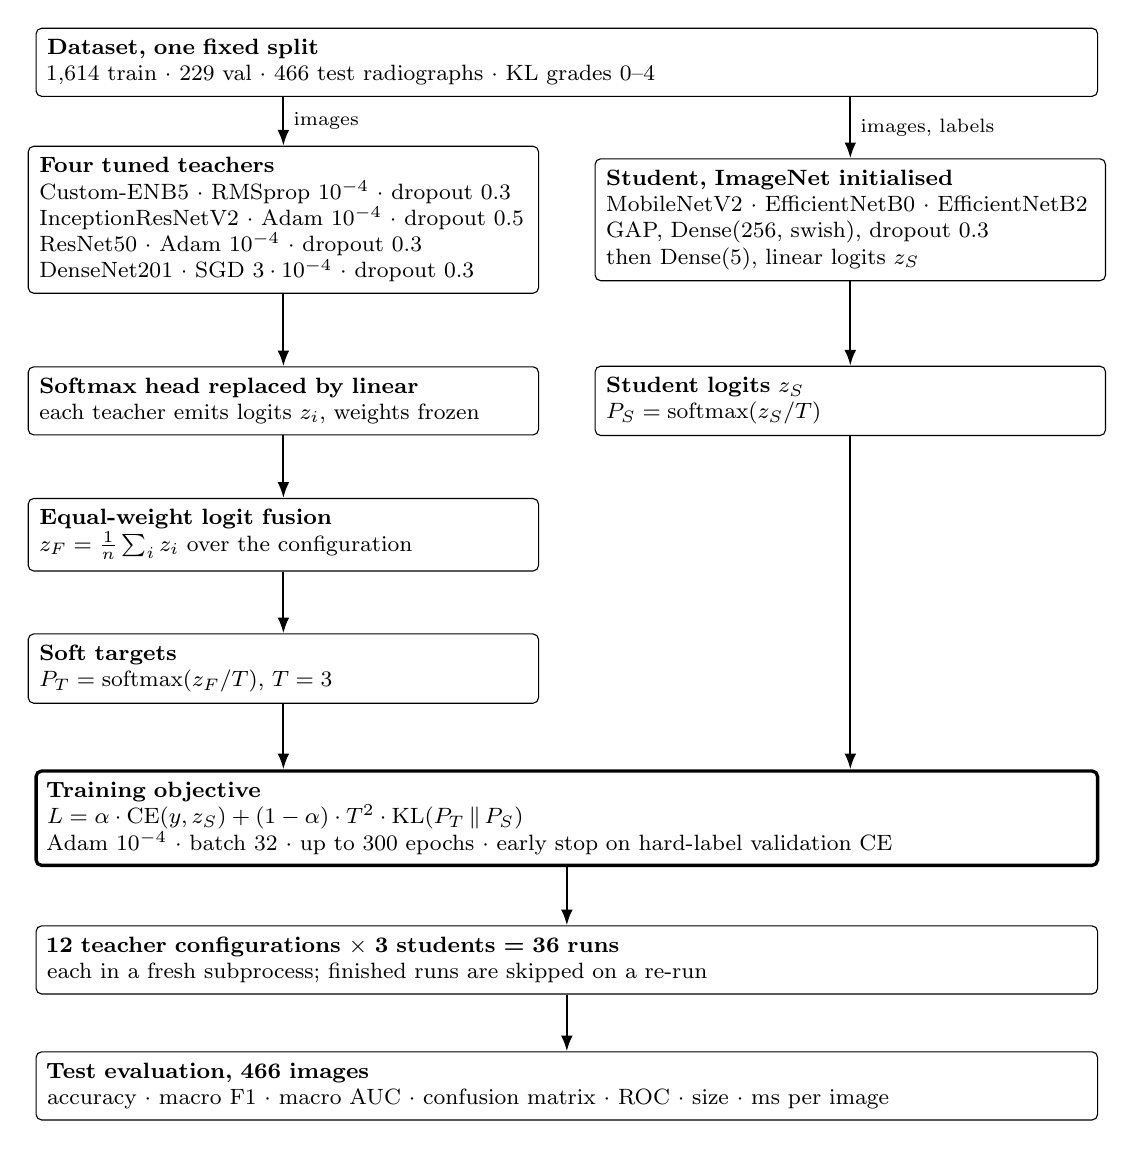
\begin{tikzpicture}[
  font=\footnotesize,
  box/.style={draw, rounded corners=2pt, align=left, inner sep=4pt, minimum height=8mm},
  wide/.style={box, text width=13.2cm},
  half/.style={box, text width=6.2cm},
  main/.style={wide, very thick},
  flow/.style={-{Latex[length=2mm]}, thick}
]
\node[wide] (data) at (0,0)
  {\textbf{Dataset, one fixed split}\\1,614 train $\cdot$ 229 val $\cdot$ 466 test radiographs $\cdot$ KL grades 0--4};
\node[half] (teach) at (-3.6,-2.0)
  {\textbf{Four tuned teachers}\\Custom-ENB5 $\cdot$ RMSprop $10^{-4}$ $\cdot$ dropout 0.3\\InceptionResNetV2 $\cdot$ Adam $10^{-4}$ $\cdot$ dropout 0.5\\ResNet50 $\cdot$ Adam $10^{-4}$ $\cdot$ dropout 0.3\\DenseNet201 $\cdot$ SGD $3\cdot10^{-4}$ $\cdot$ dropout 0.3};
\node[half] (stud) at (3.6,-2.0)
  {\textbf{Student, ImageNet initialised}\\MobileNetV2 $\cdot$ EfficientNetB0 $\cdot$ EfficientNetB2\\GAP, Dense(256, swish), dropout 0.3\\then Dense(5), linear logits $z_S$};
\node[half] (logit) at (-3.6,-4.3)
  {\textbf{Softmax head replaced by linear}\\each teacher emits logits $z_i$, weights frozen};
\node[half] (slogit) at (3.6,-4.3)
  {\textbf{Student logits} $z_S$\\$P_S=\mathrm{softmax}(z_S/T)$};
\node[half] (fuse) at (-3.6,-6.0)
  {\textbf{Equal-weight logit fusion}\\$z_F=\frac{1}{n}\sum_i z_i$ over the configuration};
\node[half] (soft) at (-3.6,-7.7)
  {\textbf{Soft targets}\\$P_T=\mathrm{softmax}(z_F/T)$, $T=3$};
\node[main] (obj) at (0,-9.6)
  {\textbf{Training objective}\\$L=\alpha\cdot\mathrm{CE}(y,z_S)+(1-\alpha)\cdot T^2\cdot\mathrm{KL}(P_T\,\|\,P_S)$\\Adam $10^{-4}$ $\cdot$ batch 32 $\cdot$ up to 300 epochs $\cdot$ early stop on hard-label validation CE};
\node[wide] (runs) at (0,-11.4)
  {\textbf{12 teacher configurations $\times$ 3 students = 36 runs}\\each in a fresh subprocess; finished runs are skipped on a re-run};
\node[wide] (eval) at (0,-13.0)
  {\textbf{Test evaluation, 466 images}\\accuracy $\cdot$ macro F1 $\cdot$ macro AUC $\cdot$ confusion matrix $\cdot$ ROC $\cdot$ size $\cdot$ ms per image};
\draw[flow] (data.south -| teach.north) -- node[right,font=\scriptsize] {images} (teach.north);
\draw[flow] (data.south -| stud.north) -- node[right,font=\scriptsize] {images, labels} (stud.north);
\draw[flow] (teach) -- (logit);
\draw[flow] (logit) -- (fuse);
\draw[flow] (fuse) -- (soft);
\draw[flow] (stud) -- (slogit);
\draw[flow] (soft.south) -- (obj.north -| soft.south);
\draw[flow] (slogit.south) -- (obj.north -| slogit.south);
\draw[flow] (obj) -- (runs);
\draw[flow] (runs) -- (eval);
\end{tikzpicture}
\caption{The distillation pipeline. The two paths meet only at the loss: teachers are never updated, they
run a forward pass on each batch, their logits are averaged, and the student pays for disagreeing with that
average as well as for getting the label wrong.}
\end{figure}
\FloatBarrier

\section{Distillation Objective}
Fusion happens in logit space. Each teacher's final softmax layer is replaced by an identical linear layer,
so teacher $i$ emits logits $z_i$ rather than probabilities. For a configuration holding $n$ teachers,

\begin{align}
z_F &= \sum_{i=1}^{n} w_i z_i, \qquad w_i = \tfrac{1}{n}, \\
L_{\mathrm{KD}} &= T^2 \cdot \mathrm{KL}\!\left(\mathrm{softmax}(z_F/T)\,\big\|\,\mathrm{softmax}(z_S/T)\right), \\
L &= \alpha \cdot \mathrm{CE}(y, z_S) + (1-\alpha) \cdot L_{\mathrm{KD}}.
\end{align}

Term by term: $z_F$ is the fused teacher opinion, averaged with equal weights because no teacher was
measurably better than the others; $T$ flattens both distributions so that the relative size of the wrong-class
probabilities, which is where a teacher's knowledge of grade similarity lives, survives the softmax; the
factor $T^2$ restores the gradient scale that dividing the logits by $T$ removed, keeping the two terms
comparable as $T$ rises; $\alpha$ is the weight on the ground truth, so $\alpha=0.3$ means 30\% hard labels
and 70\% teachers. The main grid uses $T=3$, $\alpha=0.3$; Section~\ref{sec:sweep} varies both.

Both teacher sets share Custom-ENB5 and InceptionResNetV2 and differ in the third member. Every non-empty
subset of each set is a configuration; the three shared subsets are trained once and counted for both.

\begin{table}[H]
\centering
\small
\caption{The 12 configurations. ``Control'' is the same student and recipe with hard labels only.}
\begin{tabular}{@{}llcl@{}}
\toprule
Configuration & Teachers & Count & Set \\
\midrule
none & hard labels only & 0 & control \\
D201 & DenseNet201 & 1 & A \\
ENB5 & Custom-ENB5 & 1 & A+B \\
ENB5+D201 & Custom-ENB5, DenseNet201 & 2 & A \\
ENB5+IRV2 & Custom-ENB5, InceptionResNetV2 & 2 & A+B \\
ENB5+IRV2+D201 & Custom-ENB5, InceptionResNetV2, DenseNet201 & 3 & A \\
ENB5+IRV2+R50 & Custom-ENB5, InceptionResNetV2, ResNet50 & 3 & B \\
ENB5+R50 & Custom-ENB5, ResNet50 & 2 & B \\
IRV2 & InceptionResNetV2 & 1 & A+B \\
IRV2+D201 & InceptionResNetV2, DenseNet201 & 2 & A \\
IRV2+R50 & InceptionResNetV2, ResNet50 & 2 & B \\
R50 & ResNet50 & 1 & B \\
\bottomrule
\end{tabular}
\end{table}

\section{Teachers and Fused Ensembles}
The four teachers sit within two points of each other and fusing them beats all of them. Set B gains more
from fusion than set A, which is also why set B produced the better students: a student can only inherit
what its teachers agree on.

\begin{table}[H]
\centering
\small
\caption{Teachers at their tuned settings, and the equal-weight logit fusion of each set, on the test set.}
\begin{tabular}{@{}lrrrrrr@{}}
\toprule
Model & Accuracy & Macro F1 & Weighted F1 & Macro AUC & Size (MB) & ms/image \\
\midrule
Custom-ENB5 & 0.8798 & 0.8831 & 0.8799 & 0.9746 & 247.0 & 7.8 \\
InceptionResNetV2 & 0.8734 & 0.8767 & 0.8741 & 0.9736 & 660.4 & 10.1 \\
ResNet50 & 0.8712 & 0.8750 & 0.8718 & 0.9728 & 312.4 & 3.0 \\
DenseNet201 & 0.8627 & 0.8633 & 0.8592 & 0.9737 & 168.6 & 9.0 \\
\midrule
Fused set A (ENB5+IRV2+D201) & 0.8948 & 0.8974 & 0.8946 & 0.9813 & 1076.0 & 26.8 \\
Fused set B (ENB5+IRV2+R50) & 0.9099 & 0.9121 & 0.9102 & 0.9806 & 1219.8 & 20.9 \\
\bottomrule
\end{tabular}
\end{table}

\subsection{Custom-ENB5}
\TeacherFigures{teacher_Custom-ENB5}{Custom-ENB5}

\subsection{InceptionResNetV2}
\TeacherFigures{teacher_InceptionResNetV2}{InceptionResNetV2}

\subsection{ResNet50}
\TeacherFigures{teacher_ResNet50}{ResNet50}

\subsection{DenseNet201}
\TeacherFigures{teacher_DenseNet201}{DenseNet201}

\subsection{Fused set A}
\TeacherFigures{ensemble_A}{Fused set A (ENB5+IRV2+D201)}

\subsection{Fused set B}
\TeacherFigures{ensemble_B}{Fused set B (ENB5+IRV2+R50)}

\section{Distillation Results}
Every student gains from distillation, and the smaller its own ceiling, the more it gains. The eight runs
voided by the stopping-rule artifact of Section~\ref{sec:artifact} are excluded from every aggregate below
and marked in Table~\ref{tab:all}.

\begin{table}[H]
\centering
\small
\caption{Control against the best distilled configuration for each student, macro F1.}
\begin{tabular}{@{}lrrlrr@{}}
\toprule
Student & Params (M) & Control & Best configuration & Best & Gain \\
\midrule
EfficientNetB0 & 4.38 & 0.8332 & ENB5+R50 & \textbf{0.9030} & $+$7.0 \\
EfficientNetB2 & 8.13 & 0.8584 & R50 & \textbf{0.8999} & $+$4.2 \\
MobileNetV2 & 2.59 & 0.8546 & ENB5+IRV2 & \textbf{0.8758} & $+$2.1 \\
\bottomrule
\end{tabular}
\end{table}

\begin{table}[H]
\centering
\small
\caption{Best configuration within each teacher set, macro F1. MobileNetV2's winner belongs to both sets.}
\begin{tabular}{@{}llrlr@{}}
\toprule
Student & Best in set A & Macro F1 & Best in set B & Macro F1 \\
\midrule
EfficientNetB0 & ENB5+IRV2+D201 & 0.8990 & ENB5+R50 & 0.9030 \\
EfficientNetB2 & D201 & 0.8926 & R50 & 0.8999 \\
MobileNetV2 & ENB5+IRV2 & 0.8758 & ENB5+IRV2 & 0.8758 \\
\bottomrule
\end{tabular}
\end{table}

\begin{table}[H]
\centering
\small
\caption{Averaging over the healthy distilled runs: more teachers is not better.}
\begin{tabular}{@{}crrr@{}}
\toprule
Teachers in the configuration & Runs & Mean macro F1 & Best macro F1 \\
\midrule
1 & 9 & 0.8789 & 0.8999 \\
2 & 14 & 0.8774 & 0.9030 \\
3 & 6 & 0.8775 & 0.8990 \\
\bottomrule
\end{tabular}
\end{table}

Three observations follow. First, swapping DenseNet201 for ResNet50 as the third teacher is worth
$+0.4$ points to EfficientNetB0 and $+0.7$ to EfficientNetB2. Second, the number of teachers barely moves the
mean: equal-weight averaging dilutes a strong teacher with weaker ones as readily as it combines them, and
the single best run uses two teachers while EfficientNetB2's best uses one. Third, every control stopped
early --- MobileNetV2 at 155 epochs, both EfficientNets at 83 and 84 --- while nearly every distilled run
used all 300 epochs with its best epoch at or next to the cap. The soft targets keep supplying gradient long
after hard labels stop helping, so these numbers are a floor rather than a converged result.

\begin{table}[H]
\centering
\footnotesize
\caption{Every distillation run at $T=3$, $\alpha=0.3$. Runs marked $\dagger$ were voided by the
stopping-rule artifact of Section~\ref{sec:artifact} and are excluded from all aggregates.}
\label{tab:all}
\setlength{\tabcolsep}{3.4pt}
\begin{tabular}{@{}llcrrrrrrrr@{}}
\toprule
Student & Configuration & Set & Ep./best & Val acc. & Test acc. & Macro P & Macro R & Macro F1 & AUC & Time \\
\midrule
MobileNetV2 & none & -- & 155/145 & 0.7594 & 0.8519 & 0.8589 & 0.8567 & 0.8546 & 0.9648 & 25\,m \\
MobileNetV2 & D201 & A & 300/300 & 0.8286 & 0.8476 & 0.8524 & 0.8494 & 0.8498 & 0.9681 & 49\,m \\
MobileNetV2 & ENB5$\dagger$ & A+B & 11/1 & 0.2314 & 0.2060 & 0.0704 & 0.1909 & 0.0790 & 0.5973 & 3\,m \\
MobileNetV2 & ENB5+D201 & A & 300/300 & 0.8167 & 0.8433 & 0.8614 & 0.8475 & 0.8502 & 0.9686 & 49\,m \\
MobileNetV2 & ENB5+IRV2 & A+B & 300/300 & 0.8268 & 0.8734 & 0.8750 & 0.8769 & 0.8758 & 0.9746 & 49\,m \\
MobileNetV2 & ENB5+IRV2+D201 & A & 300/299 & 0.8225 & 0.8605 & 0.8691 & 0.8629 & 0.8647 & 0.9697 & 50\,m \\
MobileNetV2 & ENB5+IRV2+R50 & B & 300/300 & 0.8318 & 0.8455 & 0.8550 & 0.8474 & 0.8499 & 0.9703 & 50\,m \\
MobileNetV2 & ENB5+R50 & B & 300/300 & 0.8261 & 0.8691 & 0.8734 & 0.8710 & 0.8718 & 0.9731 & 49\,m \\
MobileNetV2 & IRV2 & A+B & 300/300 & 0.8148 & 0.8541 & 0.8588 & 0.8563 & 0.8565 & 0.9709 & 49\,m \\
MobileNetV2 & IRV2+D201 & A & 300/300 & 0.8210 & 0.8412 & 0.8644 & 0.8470 & 0.8487 & 0.9707 & 49\,m \\
MobileNetV2 & IRV2+R50 & B & 300/300 & 0.8270 & 0.8712 & 0.8737 & 0.8751 & 0.8732 & 0.9748 & 49\,m \\
MobileNetV2 & R50$\dagger$ & B & 11/1 & 0.2402 & 0.2232 & 0.1165 & 0.2067 & 0.1000 & 0.6374 & 2\,m \\
\midrule
EfficientNetB0 & none & -- & 83/73 & 0.7875 & 0.8305 & 0.8365 & 0.8325 & 0.8332 & 0.9691 & 14\,m \\
EfficientNetB0 & D201 & A & 300/300 & 0.8323 & 0.8884 & 0.8897 & 0.8911 & 0.8895 & 0.9731 & 50\,m \\
EfficientNetB0 & ENB5$\dagger$ & A+B & 11/1 & 0.2489 & 0.2232 & 0.1352 & 0.2074 & 0.1009 & 0.6701 & 3\,m \\
EfficientNetB0 & ENB5+D201$\dagger$ & A & 11/1 & 0.2489 & 0.2146 & 0.1319 & 0.1993 & 0.0953 & 0.6278 & 4\,m \\
EfficientNetB0 & ENB5+IRV2 & A+B & 300/300 & 0.8603 & 0.8863 & 0.8910 & 0.8892 & 0.8898 & 0.9774 & 50\,m \\
EfficientNetB0 & ENB5+IRV2+D201 & A & 300/300 & 0.8601 & 0.8970 & 0.8994 & 0.8986 & 0.8990 & 0.9750 & 55\,m \\
EfficientNetB0 & ENB5+IRV2+R50 & B & 300/299 & 0.8679 & 0.8798 & 0.8831 & 0.8827 & 0.8822 & 0.9735 & 54\,m \\
EfficientNetB0 & ENB5+R50 & B & 300/300 & 0.8578 & 0.9013 & 0.9028 & 0.9039 & 0.9030 & 0.9769 & 54\,m \\
EfficientNetB0 & IRV2 & A+B & 300/300 & 0.8526 & 0.8712 & 0.8753 & 0.8728 & 0.8734 & 0.9765 & 49\,m \\
EfficientNetB0 & IRV2+D201 & A & 300/300 & 0.8616 & 0.8670 & 0.8703 & 0.8694 & 0.8683 & 0.9743 & 51\,m \\
EfficientNetB0 & IRV2+R50 & B & 300/300 & 0.8518 & 0.8820 & 0.8871 & 0.8837 & 0.8844 & 0.9766 & 54\,m \\
EfficientNetB0 & R50 & B & 300/300 & 0.8618 & 0.8691 & 0.8758 & 0.8718 & 0.8733 & 0.9722 & 53\,m \\
\midrule
EfficientNetB2 & none & -- & 84/74 & 0.8250 & 0.8541 & 0.8629 & 0.8586 & 0.8584 & 0.9676 & 16\,m \\
EfficientNetB2 & D201 & A & 300/300 & 0.8758 & 0.8906 & 0.8924 & 0.8944 & 0.8926 & 0.9756 & 53\,m \\
EfficientNetB2 & ENB5 & A+B & 300/300 & 0.8797 & 0.8884 & 0.8920 & 0.8918 & 0.8917 & 0.9737 & 53\,m \\
EfficientNetB2 & ENB5+D201 & A & 286/276 & 0.8763 & 0.8884 & 0.8903 & 0.8913 & 0.8901 & 0.9756 & 51\,m \\
EfficientNetB2 & ENB5+IRV2 & A+B & 300/298 & 0.8751 & 0.8798 & 0.8823 & 0.8814 & 0.8817 & 0.9752 & 53\,m \\
EfficientNetB2 & ENB5+IRV2+D201 & A & 300/300 & 0.8808 & 0.8734 & 0.8757 & 0.8765 & 0.8754 & 0.9742 & 54\,m \\
EfficientNetB2 & ENB5+IRV2+R50 & B & 300/295 & 0.8730 & 0.8906 & 0.8940 & 0.8938 & 0.8936 & 0.9763 & 52\,m \\
EfficientNetB2 & ENB5+R50 & B & 300/300 & 0.8831 & 0.8820 & 0.8852 & 0.8859 & 0.8839 & 0.9747 & 51\,m \\
EfficientNetB2 & IRV2 & A+B & 286/276 & 0.8731 & 0.8820 & 0.8834 & 0.8851 & 0.8839 & 0.9743 & 50\,m \\
EfficientNetB2 & IRV2+D201 & A & 300/299 & 0.8800 & 0.8798 & 0.8836 & 0.8827 & 0.8821 & 0.9781 & 52\,m \\
EfficientNetB2 & IRV2+R50 & B & 300/300 & 0.8772 & 0.8777 & 0.8830 & 0.8792 & 0.8805 & 0.9768 & 51\,m \\
EfficientNetB2 & R50 & B & 300/300 & 0.8644 & 0.8970 & 0.9014 & 0.9000 & 0.8999 & 0.9734 & 51\,m \\
\bottomrule
\end{tabular}
\end{table}
\FloatBarrier

\section{Temperature and Alpha}
\label{sec:sweep}
A $3\times3$ sweep around the winning run, EfficientNetB0 distilled from ENB5+R50, checks that $T=3$ and
$\alpha=0.3$ were not simply lucky. The $T=3$, $\alpha=0.3$ point is the main-grid run itself. Four points
were voided by the same stopping-rule artifact.

\begin{table}[H]
\centering
\small
\caption{Temperature and alpha sweep on EfficientNetB0 [ENB5+R50]. $\dagger$ marks voided runs.}
\begin{tabular}{@{}rrrrrr@{}}
\toprule
$T$ & $\alpha$ & Epochs/best & Test accuracy & Macro F1 & Macro AUC \\
\midrule
2 & 0.1 & 300/299 & 0.8734 & 0.8772 & 0.9719 \\
2 & 0.3 & 300/300 & 0.8970 & 0.8994 & 0.9754 \\
2 & 0.5 & 300/299 & 0.8584 & 0.8633 & 0.9745 \\
3$^\dagger$ & 0.1 & 11/1 & 0.2210 & 0.0913 & 0.7017 \\
3 & 0.3 & 300/300 & 0.9013 & 0.9030 & 0.9769 \\
3 & 0.5 & 300/300 & 0.9077 & \textbf{0.9095} & 0.9770 \\
5$^\dagger$ & 0.1 & 11/1 & 0.2167 & 0.0835 & 0.6931 \\
5$^\dagger$ & 0.3 & 11/1 & 0.2167 & 0.0834 & 0.6929 \\
5$^\dagger$ & 0.5 & 11/1 & 0.2189 & 0.0873 & 0.6939 \\
\bottomrule
\end{tabular}
\end{table}

The best setting is $T=3$ with $\alpha=0.5$, an even split between the teachers and the ground truth, which
lifts the headline run by a further 0.65 points. On the surviving evidence $\alpha$ matters more than $T$,
and leaning too far towards the teachers ($\alpha=0.1$ at $T=2$) costs about two points. Four of the five
missing points sit at $T=5$ or $\alpha=0.1$, so the sweep cannot yet rule on high temperature.

\subsection{The best model: EfficientNetB0 [ENB5+R50], $T=3$, $\alpha=0.5$}
\RunSummary{Custom-ENB5 + ResNet50 (set B)}{$T=3$, $\alpha=0.5$}
{4.38 M / 17.5 MB}
{300 / 300}
{0.8637}{0.9077}
{0.9095 / 0.9075}
{0.9770}{50.3 min}
\ClassificationTable{
0 & 0.9307 & 0.9307 & 0.9307 & 101 \\
1 & 0.8632 & 0.8283 & 0.8454 & 99 \\
2 & 0.8557 & 0.8830 & 0.8691 & 94 \\
3 & 0.9432 & 0.9326 & 0.9379 & 89 \\
4 & 0.9529 & 0.9759 & 0.9643 & 83 \\
Accuracy & -- & -- & 0.9077 & 466 \\
Macro average & 0.9091 & 0.9101 & 0.9095 & 466 \\
Weighted average & 0.9076 & 0.9077 & 0.9075 & 466 \\
}
\RunFigures{sweep_T3_a05}{EfficientNetB0 [ENB5+R50], $T=3$, $\alpha=0.5$}

\section{A Stopping Rule that Voided Eight Runs}
\label{sec:artifact}
Eight trainings --- four distillation runs and four sweep points --- report accuracy near 0.21 and macro F1
near 0.09, which looks like catastrophic failure. It is not: their training accuracy was already 0.83 and
still climbing when they stopped.

Validation loss is hard-label cross-entropy, and an untrained student predicts almost uniformly, so its
epoch-1 validation loss sits near $\ln 5 = 1.609$ --- low, but only because the model is undecided. The
student then becomes confident faster than it becomes accurate, validation loss climbs to about 3.0, and
needs 15 to 25 epochs to fall back under that first value. With patience counted from epoch 1, these runs
reached ten epochs without improvement at epoch 11, stopped, and \texttt{restore\_best\_weights} handed back
the undecided epoch-1 weights. The affected runs are EfficientNetB0 [ENB5], EfficientNetB0 [ENB5+D201],
MobileNetV2 [ENB5], MobileNetV2 [R50], and the sweep points at $T=3$, $\alpha=0.1$ and all three at $T=5$.

The fix is a warm-up: \texttt{start\_from\_epoch=25} makes the early epochs ineligible as the best and keeps
them out of the patience count. It was verified with patience 1 and a warm-up of 5, where the run went its
full length and selected no warm-up epoch. Because a finished \texttt{metrics.json} marks a run as done,
the eight result folders must be deleted before re-running, which costs roughly six GPU-hours. No conclusion
in this report depends on them: they can only add to the results, and one of them, MobileNetV2 [R50], may
well raise MobileNetV2's modest gain.

\section{Per-Run Results}
Every run at $T=3$, $\alpha=0.3$, grouped by student, in the order of Table~\ref{tab:all}.

\subsection{MobileNetV2}

\subsubsection{MobileNetV2 [none]}
\RunSummary{none (control)}{--}
{2.59 M / 10.4 MB}
{155 / 145}
{0.7594}{0.8519}
{0.8546 / 0.8497}
{0.9648}{24.5 min}
\ClassificationTable{
0 & 0.7607 & 0.8812 & 0.8165 & 101 \\
1 & 0.8101 & 0.6465 & 0.7191 & 99 \\
2 & 0.8416 & 0.9043 & 0.8718 & 94 \\
3 & 0.9518 & 0.8876 & 0.9186 & 89 \\
4 & 0.9302 & 0.9639 & 0.9467 & 83 \\
Accuracy & -- & -- & 0.8519 & 466 \\
Macro average & 0.8589 & 0.8567 & 0.8546 & 466 \\
Weighted average & 0.8542 & 0.8519 & 0.8497 & 466 \\
}
\RunFigures{MobileNetV2_none}{MobileNetV2 [none]}

\subsubsection{MobileNetV2 [D201]}
\RunSummary{DenseNet201}{$T=3$, $\alpha=0.3$}
{2.59 M / 10.4 MB}
{300 / 300}
{0.8286}{0.8476}
{0.8498 / 0.8473}
{0.9681}{49.2 min}
\ClassificationTable{
0 & 0.8598 & 0.9109 & 0.8846 & 101 \\
1 & 0.7451 & 0.7677 & 0.7562 & 99 \\
2 & 0.8452 & 0.7553 & 0.7978 & 94 \\
3 & 0.8632 & 0.9213 & 0.8913 & 89 \\
4 & 0.9487 & 0.8916 & 0.9193 & 83 \\
Accuracy & -- & -- & 0.8476 & 466 \\
Macro average & 0.8524 & 0.8494 & 0.8498 & 466 \\
Weighted average & 0.8490 & 0.8476 & 0.8473 & 466 \\
}
\RunFigures{MobileNetV2_D201}{MobileNetV2 [D201]}

\subsubsection{MobileNetV2 [ENB5]} \textit{Voided by the stopping-rule artifact of Section~\ref{sec:artifact}.}
\RunSummary{Custom-ENB5}{$T=3$, $\alpha=0.3$}
{2.59 M / 10.4 MB}
{11 / 1}
{0.2314}{0.2060}
{0.0790 / 0.0843}
{0.5973}{2.7 min}
\ClassificationTable{
0 & 0.2090 & 0.9208 & 0.3407 & 101 \\
1 & 0.0000 & 0.0000 & 0.0000 & 99 \\
2 & 0.0000 & 0.0000 & 0.0000 & 94 \\
3 & 0.1429 & 0.0337 & 0.0545 & 89 \\
4 & 0.0000 & 0.0000 & 0.0000 & 83 \\
Accuracy & -- & -- & 0.2060 & 466 \\
Macro average & 0.0704 & 0.1909 & 0.0790 & 466 \\
Weighted average & 0.0726 & 0.2060 & 0.0843 & 466 \\
}
\RunFigures{MobileNetV2_ENB5}{MobileNetV2 [ENB5]}

\subsubsection{MobileNetV2 [ENB5+D201]}
\RunSummary{Custom-ENB5, DenseNet201}{$T=3$, $\alpha=0.3$}
{2.59 M / 10.4 MB}
{300 / 300}
{0.8167}{0.8433}
{0.8502 / 0.8460}
{0.9686}{49.4 min}
\ClassificationTable{
0 & 0.9390 & 0.7624 & 0.8415 & 101 \\
1 & 0.6667 & 0.8485 & 0.7467 & 99 \\
2 & 0.8295 & 0.7766 & 0.8022 & 94 \\
3 & 0.9205 & 0.9101 & 0.9153 & 89 \\
4 & 0.9512 & 0.9398 & 0.9455 & 83 \\
Accuracy & -- & -- & 0.8433 & 466 \\
Macro average & 0.8614 & 0.8475 & 0.8502 & 466 \\
Weighted average & 0.8577 & 0.8433 & 0.8460 & 466 \\
}
\RunFigures{MobileNetV2_ENB5-D201}{MobileNetV2 [ENB5+D201]}

\subsubsection{MobileNetV2 [ENB5+IRV2]}
\RunSummary{Custom-ENB5, InceptionResNetV2}{$T=3$, $\alpha=0.3$}
{2.59 M / 10.4 MB}
{300 / 300}
{0.8268}{0.8734}
{0.8758 / 0.8728}
{0.9746}{49.3 min}
\ClassificationTable{
0 & 0.8824 & 0.8911 & 0.8867 & 101 \\
1 & 0.7938 & 0.7778 & 0.7857 & 99 \\
2 & 0.8462 & 0.8191 & 0.8324 & 94 \\
3 & 0.9222 & 0.9326 & 0.9274 & 89 \\
4 & 0.9302 & 0.9639 & 0.9467 & 83 \\
Accuracy & -- & -- & 0.8734 & 466 \\
Macro average & 0.8750 & 0.8769 & 0.8758 & 466 \\
Weighted average & 0.8724 & 0.8734 & 0.8728 & 466 \\
}
\RunFigures{MobileNetV2_ENB5-IRV2}{MobileNetV2 [ENB5+IRV2]}

\subsubsection{MobileNetV2 [ENB5+IRV2+D201]}
\RunSummary{Custom-ENB5, InceptionResNetV2, DenseNet201}{$T=3$, $\alpha=0.3$}
{2.59 M / 10.4 MB}
{300 / 299}
{0.8225}{0.8605}
{0.8647 / 0.8619}
{0.9697}{50.5 min}
\ClassificationTable{
0 & 0.8958 & 0.8515 & 0.8731 & 101 \\
1 & 0.7193 & 0.8283 & 0.7700 & 99 \\
2 & 0.8824 & 0.7979 & 0.8380 & 94 \\
3 & 0.9213 & 0.9213 & 0.9213 & 89 \\
4 & 0.9268 & 0.9157 & 0.9212 & 83 \\
Accuracy & -- & -- & 0.8605 & 466 \\
Macro average & 0.8691 & 0.8629 & 0.8647 & 466 \\
Weighted average & 0.8660 & 0.8605 & 0.8619 & 466 \\
}
\RunFigures{MobileNetV2_ENB5-IRV2-D201}{MobileNetV2 [ENB5+IRV2+D201]}

\subsubsection{MobileNetV2 [ENB5+IRV2+R50]}
\RunSummary{Custom-ENB5, InceptionResNetV2, ResNet50}{$T=3$, $\alpha=0.3$}
{2.59 M / 10.4 MB}
{300 / 300}
{0.8318}{0.8455}
{0.8499 / 0.8463}
{0.9703}{49.6 min}
\ClassificationTable{
0 & 0.8091 & 0.8812 & 0.8436 & 101 \\
1 & 0.7308 & 0.7677 & 0.7488 & 99 \\
2 & 0.8706 & 0.7872 & 0.8268 & 94 \\
3 & 0.8913 & 0.9213 & 0.9061 & 89 \\
4 & 0.9733 & 0.8795 & 0.9241 & 83 \\
Accuracy & -- & -- & 0.8455 & 466 \\
Macro average & 0.8550 & 0.8474 & 0.8499 & 466 \\
Weighted average & 0.8498 & 0.8455 & 0.8463 & 466 \\
}
\RunFigures{MobileNetV2_ENB5-IRV2-R50}{MobileNetV2 [ENB5+IRV2+R50]}

\subsubsection{MobileNetV2 [ENB5+R50]}
\RunSummary{Custom-ENB5, ResNet50}{$T=3$, $\alpha=0.3$}
{2.59 M / 10.4 MB}
{300 / 300}
{0.8261}{0.8691}
{0.8718 / 0.8690}
{0.9731}{49.4 min}
\ClassificationTable{
0 & 0.8598 & 0.9109 & 0.8846 & 101 \\
1 & 0.7917 & 0.7677 & 0.7795 & 99 \\
2 & 0.8316 & 0.8404 & 0.8360 & 94 \\
3 & 0.9222 & 0.9326 & 0.9274 & 89 \\
4 & 0.9615 & 0.9036 & 0.9317 & 83 \\
Accuracy & -- & -- & 0.8691 & 466 \\
Macro average & 0.8734 & 0.8710 & 0.8718 & 466 \\
Weighted average & 0.8697 & 0.8691 & 0.8690 & 466 \\
}
\RunFigures{MobileNetV2_ENB5-R50}{MobileNetV2 [ENB5+R50]}

\subsubsection{MobileNetV2 [IRV2]}
\RunSummary{InceptionResNetV2}{$T=3$, $\alpha=0.3$}
{2.59 M / 10.4 MB}
{300 / 300}
{0.8148}{0.8541}
{0.8565 / 0.8536}
{0.9709}{49.0 min}
\ClassificationTable{
0 & 0.8491 & 0.8911 & 0.8696 & 101 \\
1 & 0.8000 & 0.7273 & 0.7619 & 99 \\
2 & 0.7921 & 0.8511 & 0.8205 & 94 \\
3 & 0.8925 & 0.9326 & 0.9121 & 89 \\
4 & 0.9605 & 0.8795 & 0.9182 & 83 \\
Accuracy & -- & -- & 0.8541 & 466 \\
Macro average & 0.8588 & 0.8563 & 0.8565 & 466 \\
Weighted average & 0.8553 & 0.8541 & 0.8536 & 466 \\
}
\RunFigures{MobileNetV2_IRV2}{MobileNetV2 [IRV2]}

\subsubsection{MobileNetV2 [IRV2+D201]}
\RunSummary{InceptionResNetV2, DenseNet201}{$T=3$, $\alpha=0.3$}
{2.59 M / 10.4 MB}
{300 / 300}
{0.8210}{0.8412}
{0.8487 / 0.8433}
{0.9707}{49.2 min}
\ClassificationTable{
0 & 0.9452 & 0.6832 & 0.7931 & 101 \\
1 & 0.6462 & 0.8485 & 0.7336 & 99 \\
2 & 0.8462 & 0.8191 & 0.8324 & 94 \\
3 & 0.9326 & 0.9326 & 0.9326 & 89 \\
4 & 0.9518 & 0.9518 & 0.9518 & 83 \\
Accuracy & -- & -- & 0.8412 & 466 \\
Macro average & 0.8644 & 0.8470 & 0.8487 & 466 \\
Weighted average & 0.8605 & 0.8412 & 0.8433 & 466 \\
}
\RunFigures{MobileNetV2_IRV2-D201}{MobileNetV2 [IRV2+D201]}

\subsubsection{MobileNetV2 [IRV2+R50]}
\RunSummary{InceptionResNetV2, ResNet50}{$T=3$, $\alpha=0.3$}
{2.59 M / 10.4 MB}
{300 / 300}
{0.8270}{0.8712}
{0.8732 / 0.8702}
{0.9748}{48.8 min}
\ClassificationTable{
0 & 0.8713 & 0.8713 & 0.8713 & 101 \\
1 & 0.8295 & 0.7374 & 0.7807 & 99 \\
2 & 0.8173 & 0.9043 & 0.8586 & 94 \\
3 & 0.9412 & 0.8989 & 0.9195 & 89 \\
4 & 0.9091 & 0.9639 & 0.9357 & 83 \\
Accuracy & -- & -- & 0.8712 & 466 \\
Macro average & 0.8737 & 0.8751 & 0.8732 & 466 \\
Weighted average & 0.8716 & 0.8712 & 0.8702 & 466 \\
}
\RunFigures{MobileNetV2_IRV2-R50}{MobileNetV2 [IRV2+R50]}

\subsubsection{MobileNetV2 [R50]} \textit{Voided by the stopping-rule artifact of Section~\ref{sec:artifact}.}
\RunSummary{ResNet50}{$T=3$, $\alpha=0.3$}
{2.59 M / 10.4 MB}
{11 / 1}
{0.2402}{0.2232}
{0.1000 / 0.1070}
{0.6374}{2.4 min}
\ClassificationTable{
0 & 0.2270 & 0.9505 & 0.3664 & 101 \\
1 & 0.2222 & 0.0606 & 0.0952 & 99 \\
2 & 0.0000 & 0.0000 & 0.0000 & 94 \\
3 & 0.1333 & 0.0225 & 0.0385 & 89 \\
4 & 0.0000 & 0.0000 & 0.0000 & 83 \\
Accuracy & -- & -- & 0.2232 & 466 \\
Macro average & 0.1165 & 0.2067 & 0.1000 & 466 \\
Weighted average & 0.1219 & 0.2232 & 0.1070 & 466 \\
}
\RunFigures{MobileNetV2_R50}{MobileNetV2 [R50]}

\subsection{EfficientNetB0}

\subsubsection{EfficientNetB0 [none]}
\RunSummary{none (control)}{--}
{4.38 M / 17.5 MB}
{83 / 73}
{0.7875}{0.8305}
{0.8332 / 0.8301}
{0.9691}{13.8 min}
\ClassificationTable{
0 & 0.8198 & 0.9010 & 0.8585 & 101 \\
1 & 0.7184 & 0.7475 & 0.7327 & 99 \\
2 & 0.8519 & 0.7340 & 0.7886 & 94 \\
3 & 0.8667 & 0.8764 & 0.8715 & 89 \\
4 & 0.9259 & 0.9036 & 0.9146 & 83 \\
Accuracy & -- & -- & 0.8305 & 466 \\
Macro average & 0.8365 & 0.8325 & 0.8332 & 466 \\
Weighted average & 0.8326 & 0.8305 & 0.8301 & 466 \\
}
\RunFigures{EfficientNetB0_none}{EfficientNetB0 [none]}

\subsubsection{EfficientNetB0 [D201]}
\RunSummary{DenseNet201}{$T=3$, $\alpha=0.3$}
{4.38 M / 17.5 MB}
{300 / 300}
{0.8323}{0.8884}
{0.8895 / 0.8871}
{0.9731}{49.6 min}
\ClassificationTable{
0 & 0.8879 & 0.9406 & 0.9135 & 101 \\
1 & 0.8621 & 0.7576 & 0.8065 & 99 \\
2 & 0.8438 & 0.8617 & 0.8526 & 94 \\
3 & 0.9032 & 0.9438 & 0.9231 & 89 \\
4 & 0.9518 & 0.9518 & 0.9518 & 83 \\
Accuracy & -- & -- & 0.8884 & 466 \\
Macro average & 0.8897 & 0.8911 & 0.8895 & 466 \\
Weighted average & 0.8878 & 0.8884 & 0.8871 & 466 \\
}
\RunFigures{EfficientNetB0_D201}{EfficientNetB0 [D201]}

\subsubsection{EfficientNetB0 [ENB5]} \textit{Voided by the stopping-rule artifact of Section~\ref{sec:artifact}.}
\RunSummary{Custom-ENB5}{$T=3$, $\alpha=0.3$}
{4.38 M / 17.5 MB}
{11 / 1}
{0.2489}{0.2232}
{0.1009 / 0.1068}
{0.6701}{3.1 min}
\ClassificationTable{
0 & 0.2222 & 0.9505 & 0.3602 & 101 \\
1 & 0.0000 & 0.0000 & 0.0000 & 99 \\
2 & 0.3000 & 0.0638 & 0.1053 & 94 \\
3 & 0.1538 & 0.0225 & 0.0392 & 89 \\
4 & 0.0000 & 0.0000 & 0.0000 & 83 \\
Accuracy & -- & -- & 0.2232 & 466 \\
Macro average & 0.1352 & 0.2074 & 0.1009 & 466 \\
Weighted average & 0.1381 & 0.2232 & 0.1068 & 466 \\
}
\RunFigures{EfficientNetB0_ENB5}{EfficientNetB0 [ENB5]}

\subsubsection{EfficientNetB0 [ENB5+D201]} \textit{Voided by the stopping-rule artifact of Section~\ref{sec:artifact}.}
\RunSummary{Custom-ENB5, DenseNet201}{$T=3$, $\alpha=0.3$}
{4.38 M / 17.5 MB}
{11 / 1}
{0.2489}{0.2146}
{0.0953 / 0.1009}
{0.6278}{4.3 min}
\ClassificationTable{
0 & 0.2138 & 0.9208 & 0.3470 & 101 \\
1 & 0.0000 & 0.0000 & 0.0000 & 99 \\
2 & 0.3125 & 0.0532 & 0.0909 & 94 \\
3 & 0.1333 & 0.0225 & 0.0385 & 89 \\
4 & 0.0000 & 0.0000 & 0.0000 & 83 \\
Accuracy & -- & -- & 0.2146 & 466 \\
Macro average & 0.1319 & 0.1993 & 0.0953 & 466 \\
Weighted average & 0.1348 & 0.2146 & 0.1009 & 466 \\
}
\RunFigures{EfficientNetB0_ENB5-D201}{EfficientNetB0 [ENB5+D201]}

\subsubsection{EfficientNetB0 [ENB5+IRV2]}
\RunSummary{Custom-ENB5, InceptionResNetV2}{$T=3$, $\alpha=0.3$}
{4.38 M / 17.5 MB}
{300 / 300}
{0.8603}{0.8863}
{0.8898 / 0.8868}
{0.9774}{49.9 min}
\ClassificationTable{
0 & 0.9158 & 0.8614 & 0.8878 & 101 \\
1 & 0.8000 & 0.8485 & 0.8235 & 99 \\
2 & 0.8421 & 0.8511 & 0.8466 & 94 \\
3 & 0.9213 & 0.9213 & 0.9213 & 89 \\
4 & 0.9756 & 0.9639 & 0.9697 & 83 \\
Accuracy & -- & -- & 0.8863 & 466 \\
Macro average & 0.8910 & 0.8892 & 0.8898 & 466 \\
Weighted average & 0.8880 & 0.8863 & 0.8868 & 466 \\
}
\RunFigures{EfficientNetB0_ENB5-IRV2}{EfficientNetB0 [ENB5+IRV2]}

\subsubsection{EfficientNetB0 [ENB5+IRV2+D201]}
\RunSummary{Custom-ENB5, InceptionResNetV2, DenseNet201}{$T=3$, $\alpha=0.3$}
{4.38 M / 17.5 MB}
{300 / 300}
{0.8601}{0.8970}
{0.8990 / 0.8972}
{0.9750}{55.4 min}
\ClassificationTable{
0 & 0.9300 & 0.9208 & 0.9254 & 101 \\
1 & 0.8469 & 0.8384 & 0.8426 & 99 \\
2 & 0.8351 & 0.8617 & 0.8482 & 94 \\
3 & 0.9222 & 0.9326 & 0.9274 & 89 \\
4 & 0.9630 & 0.9398 & 0.9512 & 83 \\
Accuracy & -- & -- & 0.8970 & 466 \\
Macro average & 0.8994 & 0.8986 & 0.8990 & 466 \\
Weighted average & 0.8976 & 0.8970 & 0.8972 & 466 \\
}
\RunFigures{EfficientNetB0_ENB5-IRV2-D201}{EfficientNetB0 [ENB5+IRV2+D201]}

\subsubsection{EfficientNetB0 [ENB5+IRV2+R50]}
\RunSummary{Custom-ENB5, InceptionResNetV2, ResNet50}{$T=3$, $\alpha=0.3$}
{4.38 M / 17.5 MB}
{300 / 299}
{0.8679}{0.8798}
{0.8822 / 0.8802}
{0.9735}{53.8 min}
\ClassificationTable{
0 & 0.9451 & 0.8515 & 0.8958 & 101 \\
1 & 0.7961 & 0.8283 & 0.8119 & 99 \\
2 & 0.8469 & 0.8830 & 0.8646 & 94 \\
3 & 0.9195 & 0.8989 & 0.9091 & 89 \\
4 & 0.9080 & 0.9518 & 0.9294 & 83 \\
Accuracy & -- & -- & 0.8798 & 466 \\
Macro average & 0.8831 & 0.8827 & 0.8822 & 466 \\
Weighted average & 0.8822 & 0.8798 & 0.8802 & 466 \\
}
\RunFigures{EfficientNetB0_ENB5-IRV2-R50}{EfficientNetB0 [ENB5+IRV2+R50]}

\subsubsection{EfficientNetB0 [ENB5+R50]}
\RunSummary{Custom-ENB5, ResNet50}{$T=3$, $\alpha=0.3$}
{4.38 M / 17.5 MB}
{300 / 300}
{0.8578}{0.9013}
{0.9030 / 0.9008}
{0.9769}{54.1 min}
\ClassificationTable{
0 & 0.9118 & 0.9208 & 0.9163 & 101 \\
1 & 0.8696 & 0.8081 & 0.8377 & 99 \\
2 & 0.8485 & 0.8936 & 0.8705 & 94 \\
3 & 0.9425 & 0.9213 & 0.9318 & 89 \\
4 & 0.9419 & 0.9759 & 0.9586 & 83 \\
Accuracy & -- & -- & 0.9013 & 466 \\
Macro average & 0.9028 & 0.9039 & 0.9030 & 466 \\
Weighted average & 0.9013 & 0.9013 & 0.9008 & 466 \\
}
\RunFigures{EfficientNetB0_ENB5-R50}{EfficientNetB0 [ENB5+R50]}

\subsubsection{EfficientNetB0 [IRV2]}
\RunSummary{InceptionResNetV2}{$T=3$, $\alpha=0.3$}
{4.38 M / 17.5 MB}
{300 / 300}
{0.8526}{0.8712}
{0.8734 / 0.8718}
{0.9765}{49.3 min}
\ClassificationTable{
0 & 0.9247 & 0.8515 & 0.8866 & 101 \\
1 & 0.8037 & 0.8687 & 0.8350 & 99 \\
2 & 0.8247 & 0.8511 & 0.8377 & 94 \\
3 & 0.8953 & 0.8652 & 0.8800 & 89 \\
4 & 0.9277 & 0.9277 & 0.9277 & 83 \\
Accuracy & -- & -- & 0.8712 & 466 \\
Macro average & 0.8753 & 0.8728 & 0.8734 & 466 \\
Weighted average & 0.8738 & 0.8712 & 0.8718 & 466 \\
}
\RunFigures{EfficientNetB0_IRV2}{EfficientNetB0 [IRV2]}

\subsubsection{EfficientNetB0 [IRV2+D201]}
\RunSummary{InceptionResNetV2, DenseNet201}{$T=3$, $\alpha=0.3$}
{4.38 M / 17.5 MB}
{300 / 300}
{0.8616}{0.8670}
{0.8683 / 0.8654}
{0.9743}{51.0 min}
\ClassificationTable{
0 & 0.8319 & 0.9307 & 0.8785 & 101 \\
1 & 0.8353 & 0.7172 & 0.7717 & 99 \\
2 & 0.8421 & 0.8511 & 0.8466 & 94 \\
3 & 0.8925 & 0.9326 & 0.9121 & 89 \\
4 & 0.9500 & 0.9157 & 0.9325 & 83 \\
Accuracy & -- & -- & 0.8670 & 466 \\
Macro average & 0.8703 & 0.8694 & 0.8683 & 466 \\
Weighted average & 0.8673 & 0.8670 & 0.8654 & 466 \\
}
\RunFigures{EfficientNetB0_IRV2-D201}{EfficientNetB0 [IRV2+D201]}

\subsubsection{EfficientNetB0 [IRV2+R50]}
\RunSummary{InceptionResNetV2, ResNet50}{$T=3$, $\alpha=0.3$}
{4.38 M / 17.5 MB}
{300 / 300}
{0.8518}{0.8820}
{0.8844 / 0.8827}
{0.9766}{53.8 min}
\ClassificationTable{
0 & 0.9375 & 0.8911 & 0.9137 & 101 \\
1 & 0.8454 & 0.8283 & 0.8367 & 99 \\
2 & 0.7850 & 0.8936 & 0.8358 & 94 \\
3 & 0.9157 & 0.8539 & 0.8837 & 89 \\
4 & 0.9518 & 0.9518 & 0.9518 & 83 \\
Accuracy & -- & -- & 0.8820 & 466 \\
Macro average & 0.8871 & 0.8837 & 0.8844 & 466 \\
Weighted average & 0.8856 & 0.8820 & 0.8827 & 466 \\
}
\RunFigures{EfficientNetB0_IRV2-R50}{EfficientNetB0 [IRV2+R50]}

\subsubsection{EfficientNetB0 [R50]}
\RunSummary{ResNet50}{$T=3$, $\alpha=0.3$}
{4.38 M / 17.5 MB}
{300 / 300}
{0.8618}{0.8691}
{0.8733 / 0.8703}
{0.9722}{52.8 min}
\ClassificationTable{
0 & 0.9263 & 0.8713 & 0.8980 & 101 \\
1 & 0.7593 & 0.8283 & 0.7923 & 99 \\
2 & 0.8000 & 0.8085 & 0.8042 & 94 \\
3 & 0.9302 & 0.8989 & 0.9143 & 89 \\
4 & 0.9634 & 0.9518 & 0.9576 & 83 \\
Accuracy & -- & -- & 0.8691 & 466 \\
Macro average & 0.8758 & 0.8718 & 0.8733 & 466 \\
Weighted average & 0.8727 & 0.8691 & 0.8703 & 466 \\
}
\RunFigures{EfficientNetB0_R50}{EfficientNetB0 [R50]}

\subsection{EfficientNetB2}

\subsubsection{EfficientNetB2 [none]}
\RunSummary{none (control)}{--}
{8.13 M / 32.2 MB}
{84 / 74}
{0.8250}{0.8541}
{0.8584 / 0.8530}
{0.9676}{15.6 min}
\ClassificationTable{
0 & 0.7603 & 0.9109 & 0.8288 & 101 \\
1 & 0.7674 & 0.6667 & 0.7135 & 99 \\
2 & 0.8587 & 0.8404 & 0.8495 & 94 \\
3 & 0.9639 & 0.8989 & 0.9302 & 89 \\
4 & 0.9643 & 0.9759 & 0.9701 & 83 \\
Accuracy & -- & -- & 0.8541 & 466 \\
Macro average & 0.8629 & 0.8586 & 0.8584 & 466 \\
Weighted average & 0.8569 & 0.8541 & 0.8530 & 466 \\
}
\RunFigures{EfficientNetB2_none}{EfficientNetB2 [none]}

\subsubsection{EfficientNetB2 [D201]}
\RunSummary{DenseNet201}{$T=3$, $\alpha=0.3$}
{8.13 M / 32.2 MB}
{300 / 300}
{0.8758}{0.8906}
{0.8926 / 0.8893}
{0.9756}{52.8 min}
\ClassificationTable{
0 & 0.8774 & 0.9208 & 0.8986 & 101 \\
1 & 0.8409 & 0.7475 & 0.7914 & 99 \\
2 & 0.8469 & 0.8830 & 0.8646 & 94 \\
3 & 0.9432 & 0.9326 & 0.9379 & 89 \\
4 & 0.9535 & 0.9880 & 0.9704 & 83 \\
Accuracy & -- & -- & 0.8906 & 466 \\
Macro average & 0.8924 & 0.8944 & 0.8926 & 466 \\
Weighted average & 0.8896 & 0.8906 & 0.8893 & 466 \\
}
\RunFigures{EfficientNetB2_D201}{EfficientNetB2 [D201]}

\subsubsection{EfficientNetB2 [ENB5]}
\RunSummary{Custom-ENB5}{$T=3$, $\alpha=0.3$}
{8.13 M / 32.2 MB}
{300 / 300}
{0.8797}{0.8884}
{0.8917 / 0.8882}
{0.9737}{52.7 min}
\ClassificationTable{
0 & 0.8667 & 0.9010 & 0.8835 & 101 \\
1 & 0.8021 & 0.7778 & 0.7897 & 99 \\
2 & 0.8737 & 0.8830 & 0.8783 & 94 \\
3 & 0.9647 & 0.9213 & 0.9425 & 89 \\
4 & 0.9529 & 0.9759 & 0.9643 & 83 \\
Accuracy & -- & -- & 0.8884 & 466 \\
Macro average & 0.8920 & 0.8918 & 0.8917 & 466 \\
Weighted average & 0.8885 & 0.8884 & 0.8882 & 466 \\
}
\RunFigures{EfficientNetB2_ENB5}{EfficientNetB2 [ENB5]}

\subsubsection{EfficientNetB2 [ENB5+D201]}
\RunSummary{Custom-ENB5, DenseNet201}{$T=3$, $\alpha=0.3$}
{8.13 M / 32.2 MB}
{286 / 276}
{0.8763}{0.8884}
{0.8901 / 0.8876}
{0.9756}{50.8 min}
\ClassificationTable{
0 & 0.8846 & 0.9109 & 0.8976 & 101 \\
1 & 0.8539 & 0.7677 & 0.8085 & 99 \\
2 & 0.8400 & 0.8936 & 0.8660 & 94 \\
3 & 0.9326 & 0.9326 & 0.9326 & 89 \\
4 & 0.9405 & 0.9518 & 0.9461 & 83 \\
Accuracy & -- & -- & 0.8884 & 466 \\
Macro average & 0.8903 & 0.8913 & 0.8901 & 466 \\
Weighted average & 0.8882 & 0.8884 & 0.8876 & 466 \\
}
\RunFigures{EfficientNetB2_ENB5-D201}{EfficientNetB2 [ENB5+D201]}

\subsubsection{EfficientNetB2 [ENB5+IRV2]}
\RunSummary{Custom-ENB5, InceptionResNetV2}{$T=3$, $\alpha=0.3$}
{8.13 M / 32.2 MB}
{300 / 298}
{0.8751}{0.8798}
{0.8817 / 0.8799}
{0.9752}{52.8 min}
\ClassificationTable{
0 & 0.9010 & 0.9010 & 0.9010 & 101 \\
1 & 0.8081 & 0.8081 & 0.8081 & 99 \\
2 & 0.8526 & 0.8617 & 0.8571 & 94 \\
3 & 0.9121 & 0.9326 & 0.9222 & 89 \\
4 & 0.9375 & 0.9036 & 0.9202 & 83 \\
Accuracy & -- & -- & 0.8798 & 466 \\
Macro average & 0.8823 & 0.8814 & 0.8817 & 466 \\
Weighted average & 0.8801 & 0.8798 & 0.8799 & 466 \\
}
\RunFigures{EfficientNetB2_ENB5-IRV2}{EfficientNetB2 [ENB5+IRV2]}

\subsubsection{EfficientNetB2 [ENB5+IRV2+D201]}
\RunSummary{Custom-ENB5, InceptionResNetV2, DenseNet201}{$T=3$, $\alpha=0.3$}
{8.13 M / 32.2 MB}
{300 / 300}
{0.8808}{0.8734}
{0.8754 / 0.8723}
{0.9742}{54.0 min}
\ClassificationTable{
0 & 0.8598 & 0.9109 & 0.8846 & 101 \\
1 & 0.8202 & 0.7374 & 0.7766 & 99 \\
2 & 0.8351 & 0.8617 & 0.8482 & 94 \\
3 & 0.9121 & 0.9326 & 0.9222 & 89 \\
4 & 0.9512 & 0.9398 & 0.9455 & 83 \\
Accuracy & -- & -- & 0.8734 & 466 \\
Macro average & 0.8757 & 0.8765 & 0.8754 & 466 \\
Weighted average & 0.8727 & 0.8734 & 0.8723 & 466 \\
}
\RunFigures{EfficientNetB2_ENB5-IRV2-D201}{EfficientNetB2 [ENB5+IRV2+D201]}

\subsubsection{EfficientNetB2 [ENB5+IRV2+R50]}
\RunSummary{Custom-ENB5, InceptionResNetV2, ResNet50}{$T=3$, $\alpha=0.3$}
{8.13 M / 32.2 MB}
{300 / 295}
{0.8730}{0.8906}
{0.8936 / 0.8908}
{0.9763}{52.0 min}
\ClassificationTable{
0 & 0.9167 & 0.8713 & 0.8934 & 101 \\
1 & 0.8039 & 0.8283 & 0.8159 & 99 \\
2 & 0.8542 & 0.8723 & 0.8632 & 94 \\
3 & 0.9535 & 0.9213 & 0.9371 & 89 \\
4 & 0.9419 & 0.9759 & 0.9586 & 83 \\
Accuracy & -- & -- & 0.8906 & 466 \\
Macro average & 0.8940 & 0.8938 & 0.8936 & 466 \\
Weighted average & 0.8916 & 0.8906 & 0.8908 & 466 \\
}
\RunFigures{EfficientNetB2_ENB5-IRV2-R50}{EfficientNetB2 [ENB5+IRV2+R50]}

\subsubsection{EfficientNetB2 [ENB5+R50]}
\RunSummary{Custom-ENB5, ResNet50}{$T=3$, $\alpha=0.3$}
{8.13 M / 32.2 MB}
{300 / 300}
{0.8831}{0.8820}
{0.8839 / 0.8803}
{0.9747}{51.1 min}
\ClassificationTable{
0 & 0.8440 & 0.9109 & 0.8762 & 101 \\
1 & 0.8452 & 0.7172 & 0.7760 & 99 \\
2 & 0.8416 & 0.9043 & 0.8718 & 94 \\
3 & 0.9535 & 0.9213 & 0.9371 & 89 \\
4 & 0.9419 & 0.9759 & 0.9586 & 83 \\
Accuracy & -- & -- & 0.8820 & 466 \\
Macro average & 0.8852 & 0.8859 & 0.8839 & 466 \\
Weighted average & 0.8821 & 0.8820 & 0.8803 & 466 \\
}
\RunFigures{EfficientNetB2_ENB5-R50}{EfficientNetB2 [ENB5+R50]}

\subsubsection{EfficientNetB2 [IRV2]}
\RunSummary{InceptionResNetV2}{$T=3$, $\alpha=0.3$}
{8.13 M / 32.2 MB}
{286 / 276}
{0.8731}{0.8820}
{0.8839 / 0.8816}
{0.9743}{50.4 min}
\ClassificationTable{
0 & 0.9082 & 0.8812 & 0.8945 & 101 \\
1 & 0.8404 & 0.7980 & 0.8187 & 99 \\
2 & 0.8283 & 0.8723 & 0.8497 & 94 \\
3 & 0.9205 & 0.9101 & 0.9153 & 89 \\
4 & 0.9195 & 0.9639 & 0.9412 & 83 \\
Accuracy & -- & -- & 0.8820 & 466 \\
Macro average & 0.8834 & 0.8851 & 0.8839 & 466 \\
Weighted average & 0.8820 & 0.8820 & 0.8816 & 466 \\
}
\RunFigures{EfficientNetB2_IRV2}{EfficientNetB2 [IRV2]}

\subsubsection{EfficientNetB2 [IRV2+D201]}
\RunSummary{InceptionResNetV2, DenseNet201}{$T=3$, $\alpha=0.3$}
{8.13 M / 32.2 MB}
{300 / 299}
{0.8800}{0.8798}
{0.8821 / 0.8800}
{0.9781}{52.4 min}
\ClassificationTable{
0 & 0.9167 & 0.8713 & 0.8934 & 101 \\
1 & 0.8020 & 0.8182 & 0.8100 & 99 \\
2 & 0.8469 & 0.8830 & 0.8646 & 94 \\
3 & 0.9625 & 0.8652 & 0.9112 & 89 \\
4 & 0.8901 & 0.9759 & 0.9310 & 83 \\
Accuracy & -- & -- & 0.8798 & 466 \\
Macro average & 0.8836 & 0.8827 & 0.8821 & 466 \\
Weighted average & 0.8823 & 0.8798 & 0.8800 & 466 \\
}
\RunFigures{EfficientNetB2_IRV2-D201}{EfficientNetB2 [IRV2+D201]}

\subsubsection{EfficientNetB2 [IRV2+R50]}
\RunSummary{InceptionResNetV2, ResNet50}{$T=3$, $\alpha=0.3$}
{8.13 M / 32.2 MB}
{300 / 300}
{0.8772}{0.8777}
{0.8805 / 0.8786}
{0.9768}{51.0 min}
\ClassificationTable{
0 & 0.9263 & 0.8713 & 0.8980 & 101 \\
1 & 0.7736 & 0.8283 & 0.8000 & 99 \\
2 & 0.8542 & 0.8723 & 0.8632 & 94 \\
3 & 0.9121 & 0.9326 & 0.9222 & 89 \\
4 & 0.9487 & 0.8916 & 0.9193 & 83 \\
Accuracy & -- & -- & 0.8777 & 466 \\
Macro average & 0.8830 & 0.8792 & 0.8805 & 466 \\
Weighted average & 0.8806 & 0.8777 & 0.8786 & 466 \\
}
\RunFigures{EfficientNetB2_IRV2-R50}{EfficientNetB2 [IRV2+R50]}

\subsubsection{EfficientNetB2 [R50]}
\RunSummary{ResNet50}{$T=3$, $\alpha=0.3$}
{8.13 M / 32.2 MB}
{300 / 300}
{0.8644}{0.8970}
{0.8999 / 0.8971}
{0.9734}{51.0 min}
\ClassificationTable{
0 & 0.9000 & 0.8911 & 0.8955 & 101 \\
1 & 0.8265 & 0.8182 & 0.8223 & 99 \\
2 & 0.8515 & 0.9149 & 0.8821 & 94 \\
3 & 0.9753 & 0.8876 & 0.9294 & 89 \\
4 & 0.9535 & 0.9880 & 0.9704 & 83 \\
Accuracy & -- & -- & 0.8970 & 466 \\
Macro average & 0.9014 & 0.9000 & 0.8999 & 466 \\
Weighted average & 0.8985 & 0.8970 & 0.8971 & 466 \\
}
\RunFigures{EfficientNetB2_R50}{EfficientNetB2 [R50]}

\section{Comparison Figures}
\begin{figure}[H]
\centering
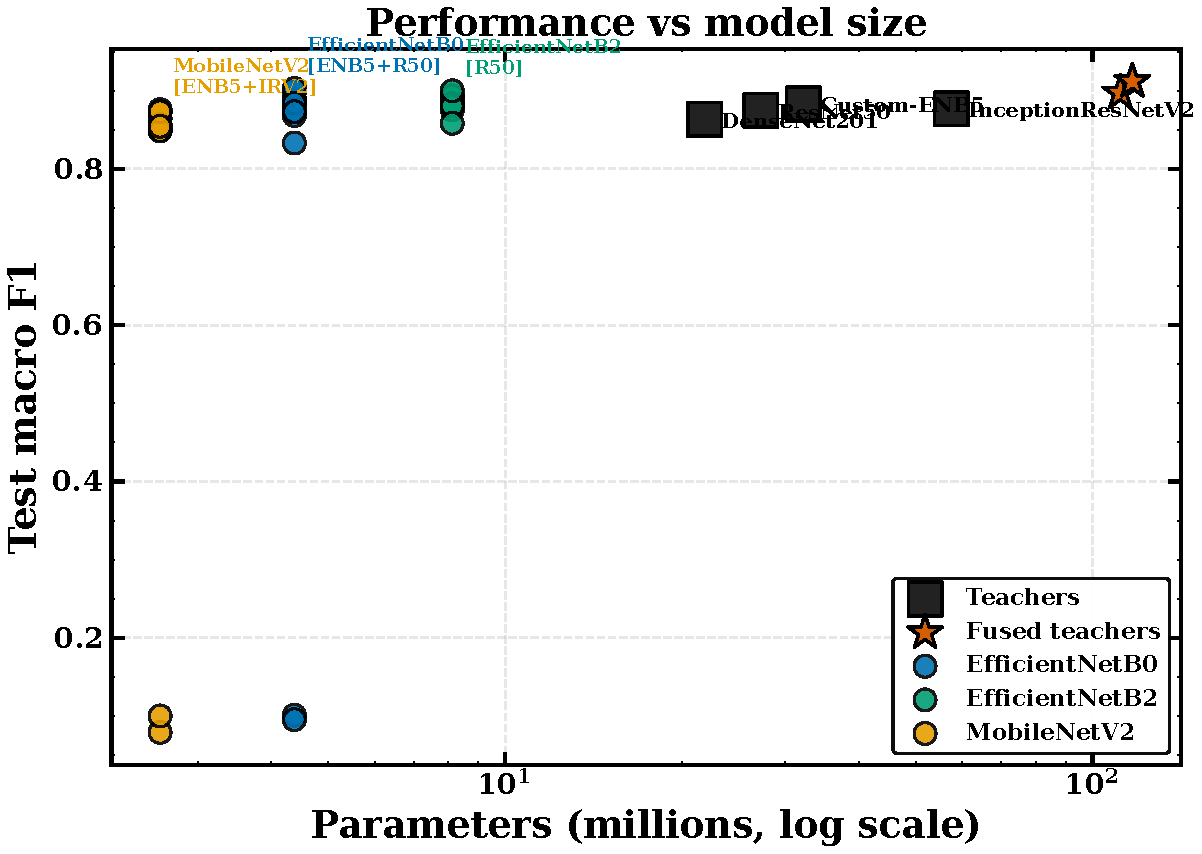
\includegraphics[width=0.92\textwidth]{summary_performance_vs_size.pdf}
\caption{Test macro F1 against on-disk size. The distilled students occupy the upper-left corner: the
accuracy of the ensemble at a fraction of its footprint.}
\end{figure}

\begin{figure}[H]
\centering
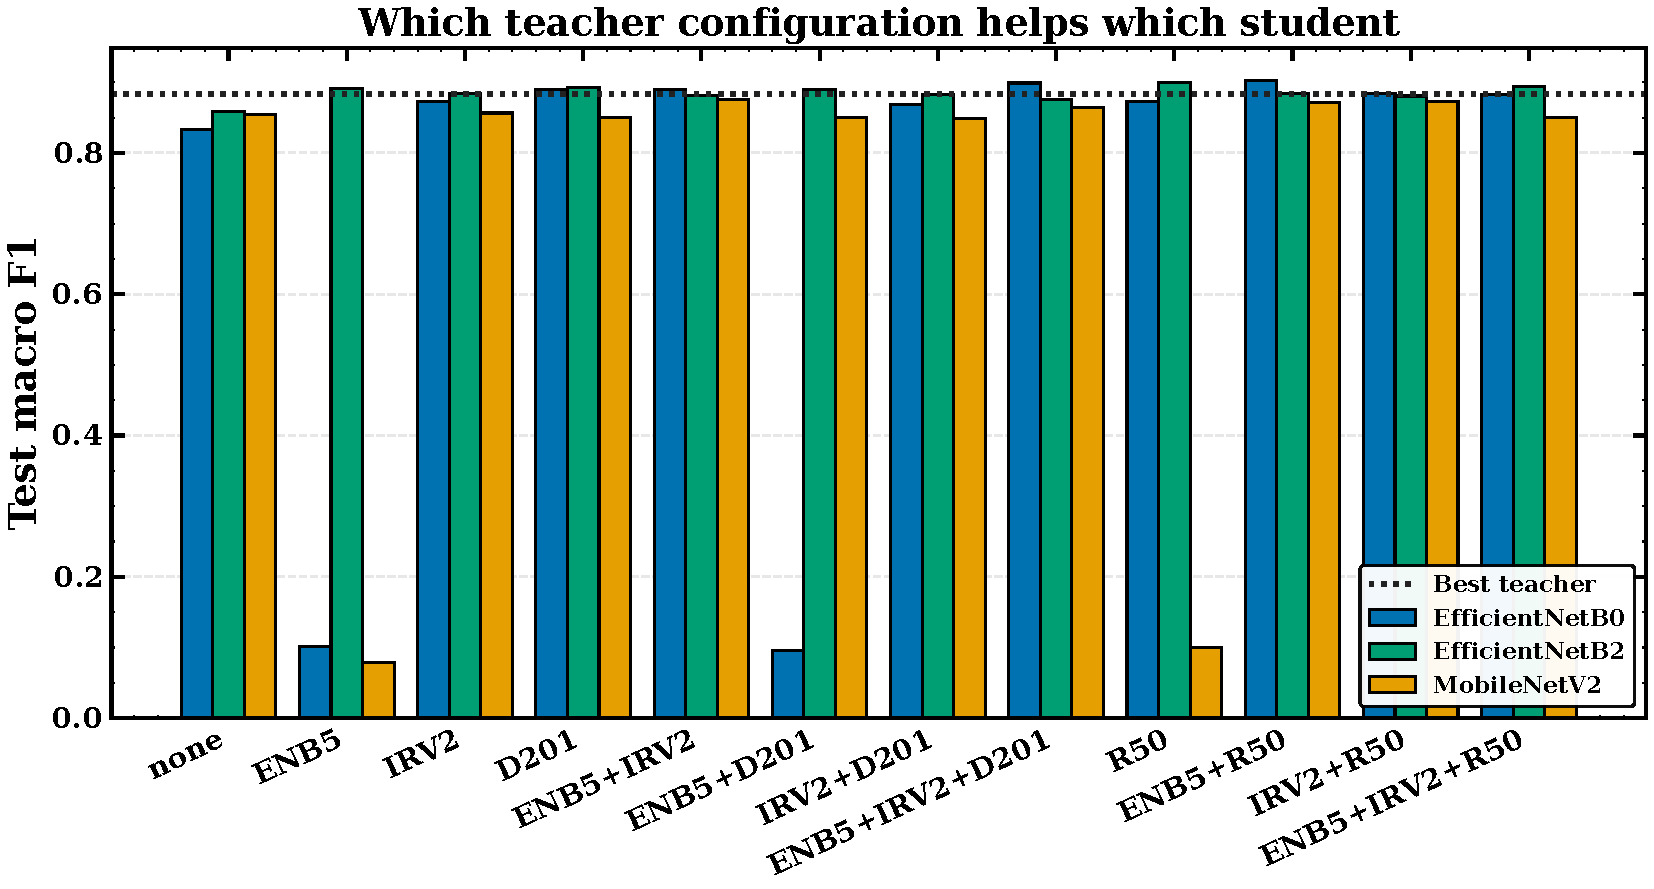
\includegraphics[width=0.92\textwidth]{summary_teacher_vs_student.pdf}
\caption{Teachers, fused ensembles, and the students distilled from them.}
\end{figure}

\begin{figure}[H]
\centering
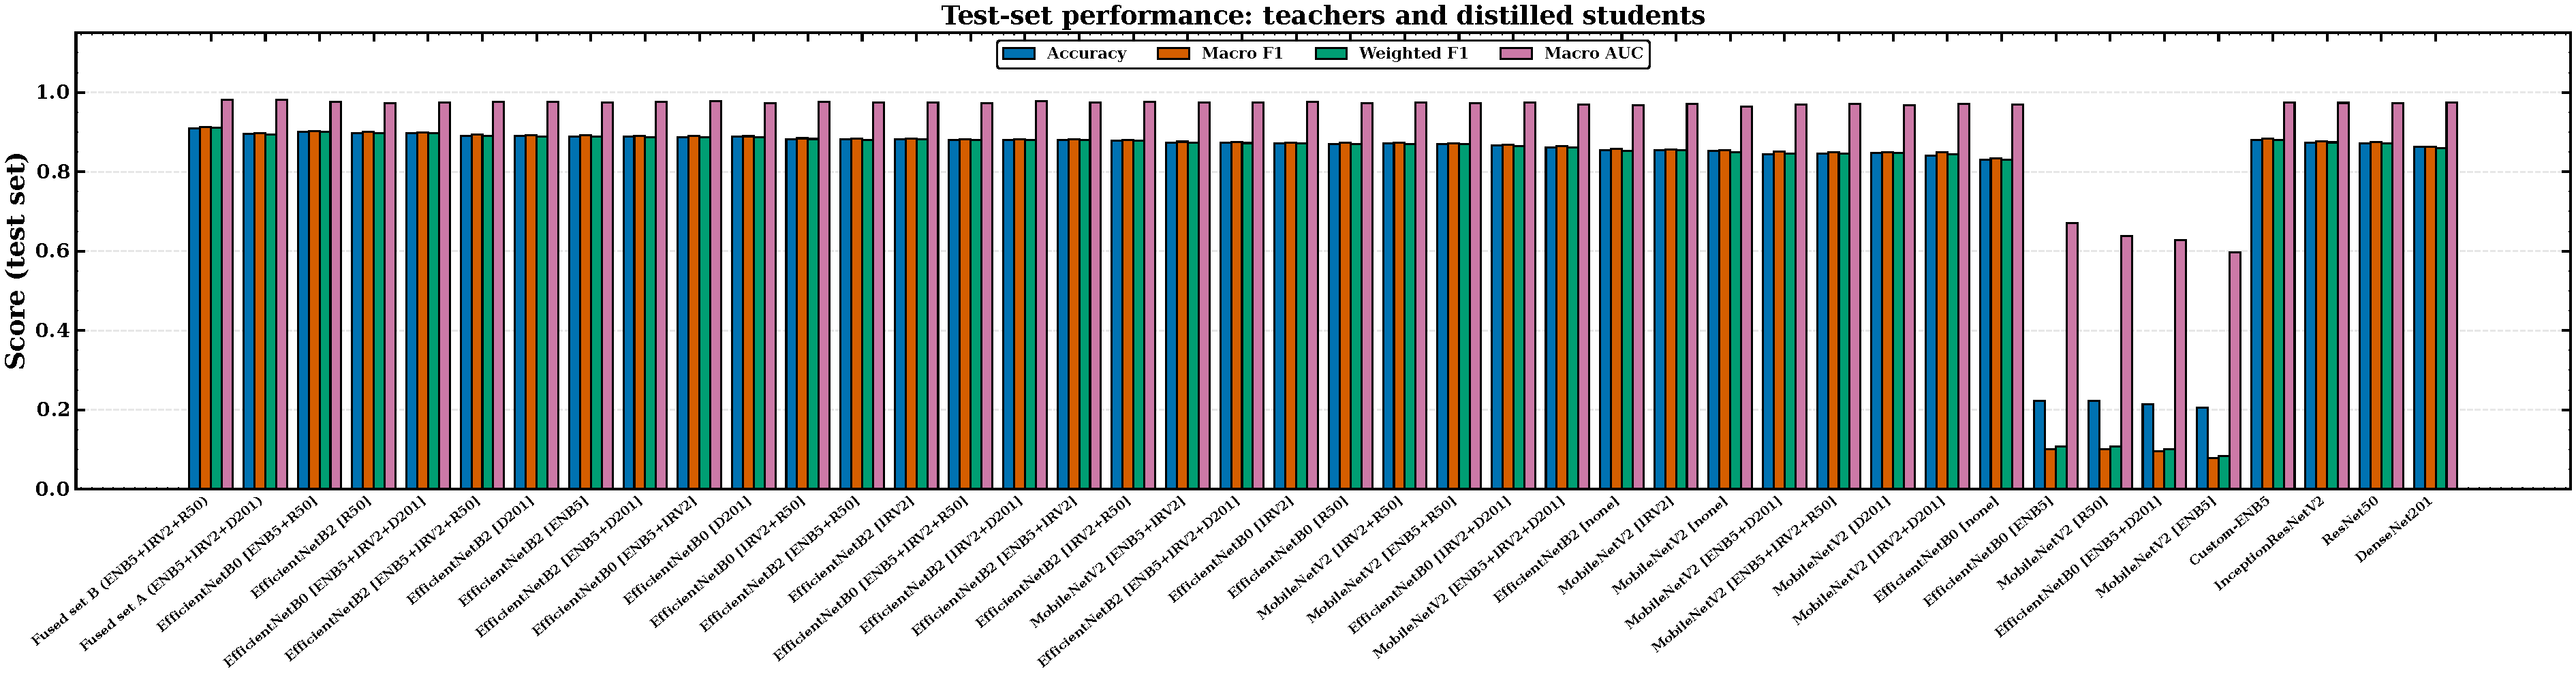
\includegraphics[width=0.92\textwidth]{summary_test_metrics.pdf}
\caption{Test-set metrics across every model in the study.}
\end{figure}

\begin{figure}[H]
\centering
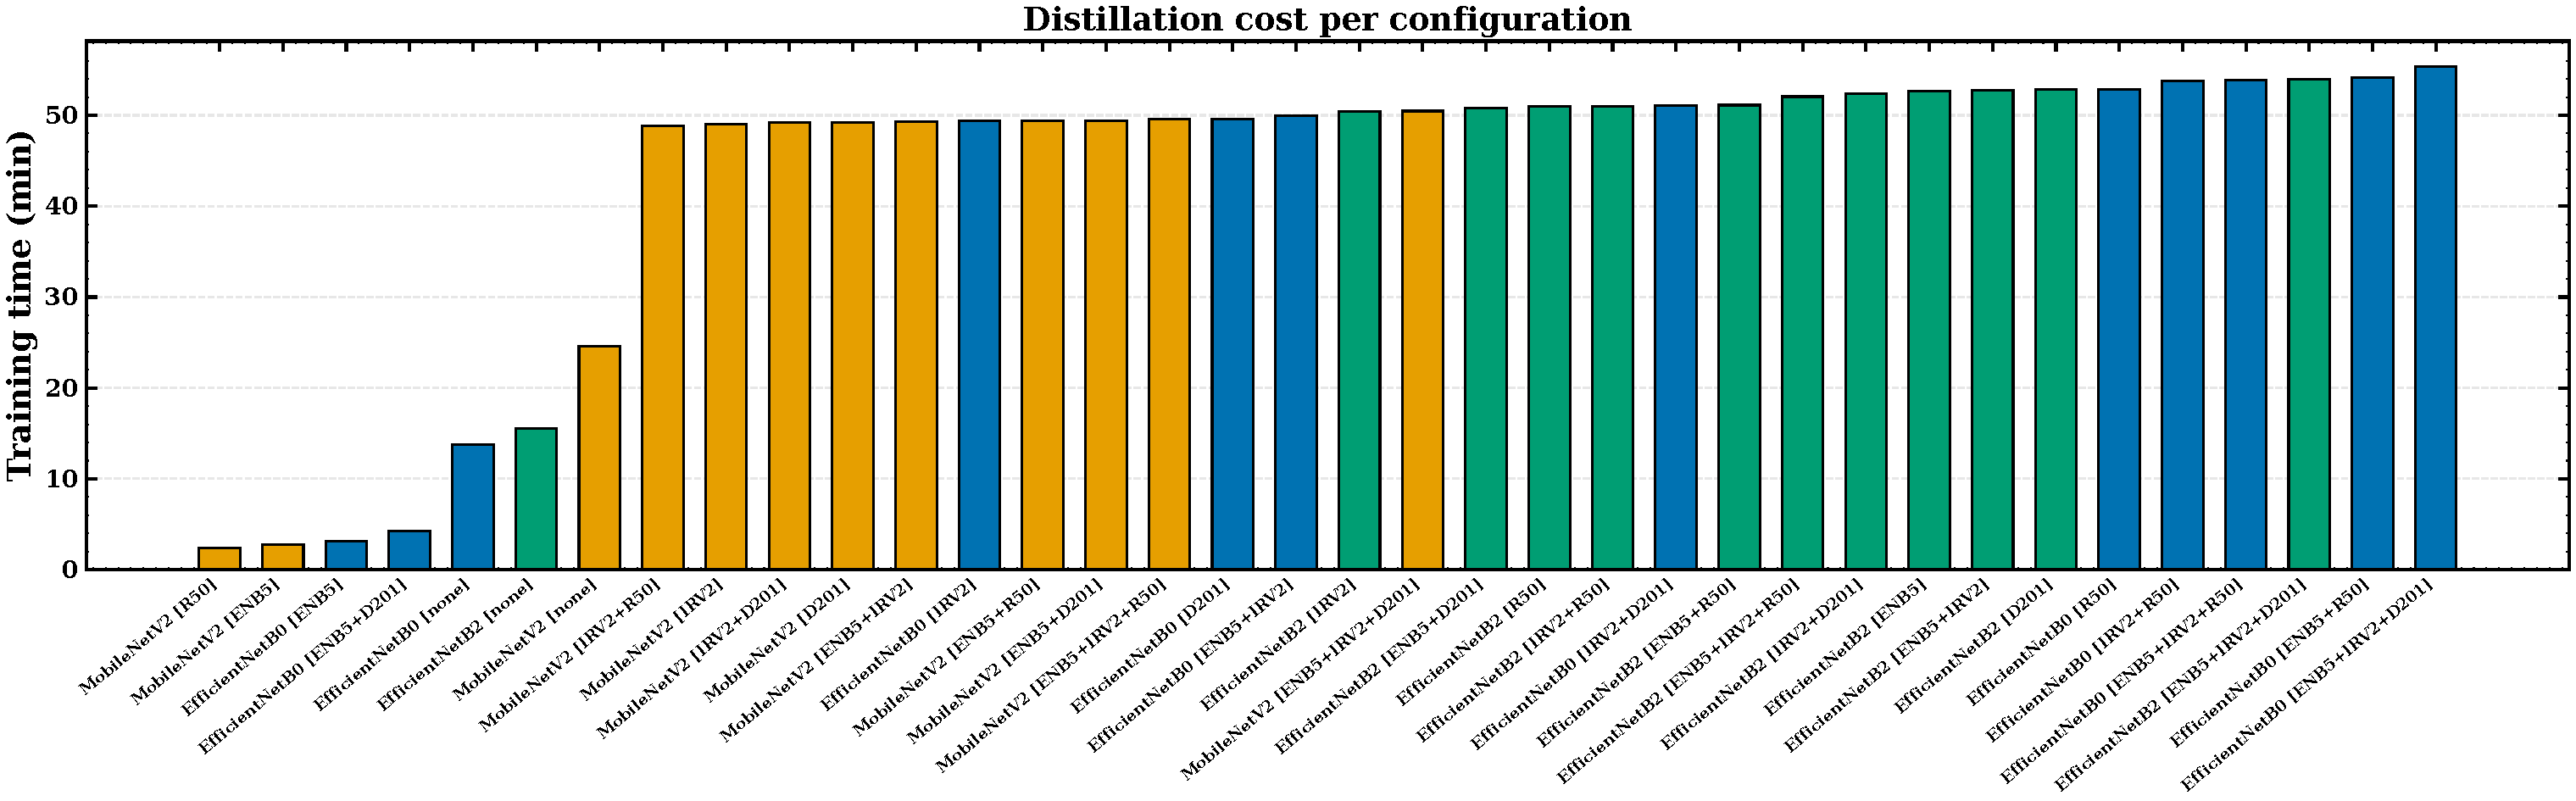
\includegraphics[width=0.92\textwidth]{summary_training_time.pdf}
\caption{Training time per run. Distilled runs cost more per epoch, because every teacher runs a forward
pass on each batch, and they also use far more epochs before early stopping fires.}
\end{figure}

\begin{figure}[H]
\centering
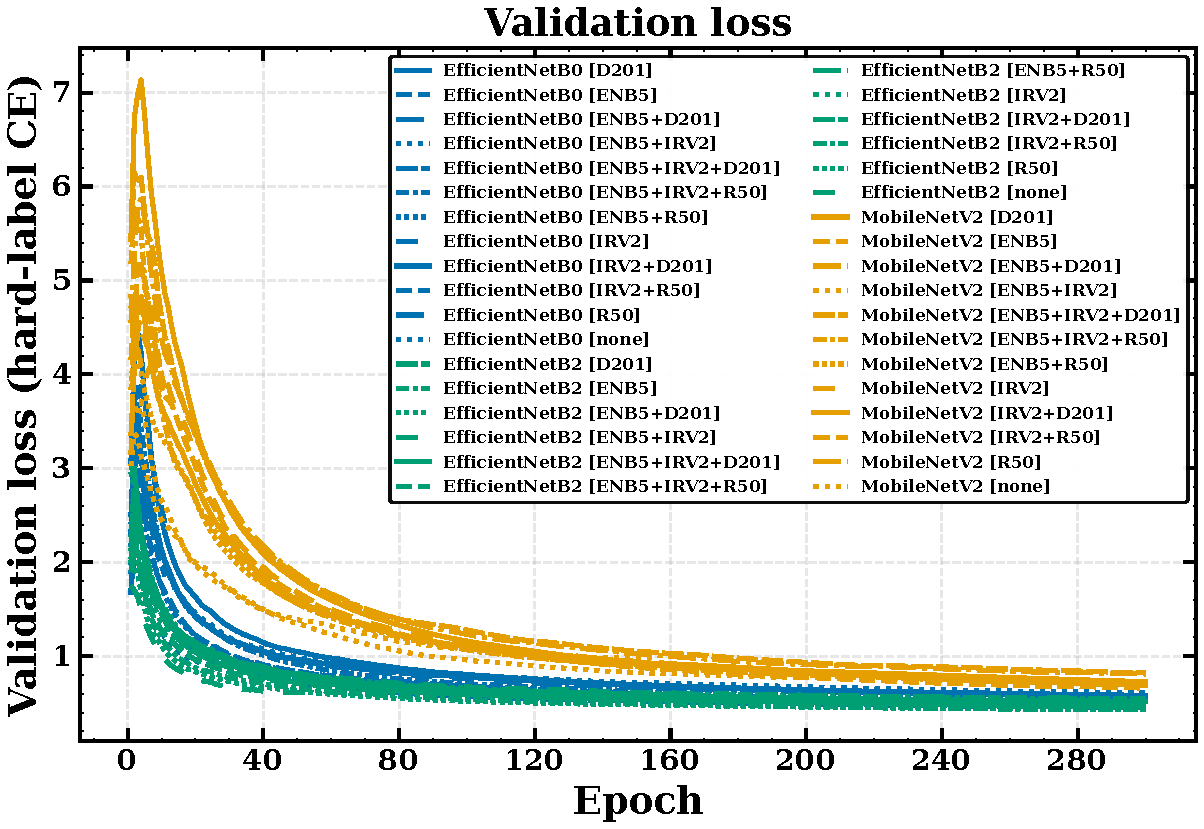
\includegraphics[width=0.92\textwidth]{summary_val_loss_all.pdf}
\caption{Hard-label validation loss for every run. The voided runs are the curves that stop at epoch 11.}
\end{figure}
\FloatBarrier

\section{Reproducing the Results}
The notebook \texttt{kd/KD\_MultiTeacher\_Distillation.ipynb} produces every number and figure in this
report, writing one folder per run under \texttt{kd/results/} with \texttt{metrics.json},
\texttt{history.csv}, the classification report, the confusion matrix, per-image predictions, the student
weights, and vector plus 600\,dpi figures. To re-train the eight voided runs with the warm-up fix, delete
their folders and re-run the notebook: finished runs are reloaded from disk and only the deleted ones are
trained again.

\end{document}
